% Tutamen: A Second-Generation Secret Storage as a Service Platform
% Paper
%
% 2016
%
% Andy Sayler
% Taylor Andrews
% Matt Monaco
% Dirk Grunwald

% SoCC Template: do not change these values
\documentclass[10pt,twocolumn]{article}
\usepackage{times}
\baselineskip 12pt
\textheight 9in
\textwidth 6.5in
\oddsidemargin 0in
\topmargin 0in
\headheight 0in
\headsep 0in

% System Packages
\usepackage{epsfig}
\usepackage{float}
\usepackage{caption}
\usepackage{subcaption}
\usepackage{tabu}
\usepackage{color}
\usepackage{hyperref}
\usepackage{url}
\usepackage{listings}
\usepackage{authblk}

% Package Options
\hypersetup{
    colorlinks,
    citecolor=black,
    filecolor=black,
    linkcolor=black,
    urlcolor=black
}

% Macros
\input{macros.tex}

% Other Options
\clubpenalty = 10000
\widowpenalty = 10000

% Start
\begin{document}

%make title bold and 14 pt font (Latex default is non-bold, 16 pt)
\title{Tutamen: A Next-Generation Secret-Storage Platform}

% start author
\author{Andy Sayler}
\author{Taylor Andrews}
\author{Matt Monaco}
\author{Dirk Grunwald}
\affil{University of Colorado}
% end author

%don't want date printed
\date{}

\maketitle

\begin{abstract}
The storage and management of secrets (encryption keys, passwords,
etc) are significant open problems in the modern age of cloud-based,
third-party hosted, ephemeral computing infrastructure. How do we
store and control access to the secrets necessary to configure and
operate a range of modern technologies without sacrificing security
and privacy requirements or significantly curtailing the desirable
capabilities of our applications? To answer this question, we propose
Tutamen -- a next generation secret storage service. Tutamen offers a
number of desirable properties not present in existing secret storage
solutions. These include the ability to operate atop minimally trusted
infrastructure and the ability to control secret access based on
contextual, multi-factor, and alternate-band authentication
parameters. These properties have allowed us to leverage Tutamen to
support a variety of use cases not easily realizable using existing
systems, including supporting full-disk encryption on headless servers
and providing fully-featured client-side encryption to cloud-based
file lockers. We present the importance of the secret storage problem,
Tutamen's design and architecture, the implementation of our Tutamen
prototype, and several of the applications in which we have
implemented Tutamen-based secret storage to achieve previously
unattainable goals while still meeting a variety of security and
privacy requirements.
\end{abstract}

\section{Introduction}
\label{sec:intro}

How best to store and manage secrets -- the bits of tightly controlled
data necessary to ensure or bootstrap the security of computing
systems and services -- has always been a non-trivial problem. As we
continue to move toward computing and storage platforms controlled by
third parties, and embrace modern trends toward ephemeral
infrastructure, the secret-storage problem only becomes more prevalent
and critical to solve.

Tutamen\footnote{Latin -- A means of protection or defense.} is our
attempt to solve the secret-storage problem in a manner that allows
the user to adhere to a range of security and privacy requirements
without sacrificing functionality in the process. Tutamen is a next
generation secret-storage platform. It builds on our previous secret
storage efforts~\cite{custos-trios} and strives to offer features not
provided by the various secret-storage systems available today. In
this paper, we offer several contributions:

\begin{packed_item}
\item The design, implementation, and evaluation of a secret-storage
  system with support for several novel features, including:
  \begin{packed_item}
  \item Modular authentication modules designed to add flexibility
    through the use of contextual, multi-factor, and alternate-band
    (e.g., SMS text messages) authentication mechanisms.
  \item The ability to operate atop minimally trusted infrastructure
    by leveraging multiple storage and access control providers to
    achieve both redundancy and to mitigate trust.
  \end{packed_item}
\item Several practical demonstrations of how a secret-storage system
  with such features can be integrated with real-world applications to
  offer desirable features in a secure and easy-to-use manner.
\end{packed_item}

\subsection{The Need for Secret-Storage}

Computing systems today invade every contour of our lives -- from the
fitness trackers on our wrists, to our ``smart'' home appliances, to
the server infrastructure required to support the range of web sites
and services we interact with every day. With this explosion of
computing systems has come an equally large explosion in the amount of
data stored by and about us. While some of this data is designed to be
public (i.e., the entries on Wikipedia), much of it is not, requiring
the enforcement of various privacy and security guarantees with
respect to its handling and storage. The basis of providing such
guarantees relies on our ability to store and selectively share
secrets ranging from the keys used to encrypt our data to the
passwords used to protect our online accounts. How best to store and
manage these secrets is thus a critical question -- the answer to
which forms the foundation to all of computing's higher level security
and privacy guarantees.

Beyond the need to bootstrap a variety of security guarantees, there
are several other factors driving the need for robust secret storage
solutions. On the system administration front, the trend toward
ephemeral infrastructure capable of rapidly scaling up or down is
driving the adoption of configuration management systems such as
Puppet~\cite{puppet} or Chef~\cite{chef}. Such systems, however, do
not tend to have suitable mechanisms for enforcing the security and
privacy requirements inherent to storing secrets. Despite this,
configuration data often contains a variety of secrets such as SSH
keys, TLS/SSL keys, file encryption keys, and the tokens or
credentials necessary to authenticate with external APIs and services.

Similarly, on the end user front, the need for suitable secret-storage
systems is being driven by a rapid expansion of the number of sites
and services to which users must authenticate themselves, as well as
by the growing expanse of digital data users wish to protect. Indeed,
the popularity of password management systems such as
LastPass~\cite{lastpass} or 1Password~\cite{onepassword} as well as
user and manufacturer demands for encryption support on their
devices~\cite{apple-fbiletter} demonstrate the importance of secret
storage, and the applications it enables, to end users.

\subsection{The Ideal Secret-Storage System}

Unlike standard configuration management systems, or even specific
secret-storage systems such as password managers, a general purpose
secret-storage presents a number of unique requirements, including the
following capabilities:

\begin{packed_item}
\item Store a wide-range of arbitrary secret data
\item Store secret data in a secure manner
\item Enforce fine-grained access control requirements
\item Support a range of authentication sources/methods
\item Provide audit logs tracking secret access history
\end{packed_item}

In response to these needs, a number of general purpose secret-storage
systems have been recently developed by industry, including
HashiCorp's Vault~\cite{vault}, Lyft's Confidant~\cite{confidant}, and
Square's Keywhiz~\cite{keywhiz}. These systems exist to fulfill some
or all of the requirements listed above. We believe, however, that
such systems are hindered by several key limitations. First, they
generally require at least one fully trusted server as the basis of
their security model, making them unsuitable for operation atop
untrusted infrastructure. Second, they tend to lack support for use
cases requiring autonomous or remote access to secret material in a
secure manner. These deficiencies give rise to a few more secret
storage requirements:

\begin{packed_item}
\item Avoidance of the need to place a high degree of trust in any
  single system outside the application that wishes to store a secret.
\item Ability to support a range of secret access use cases, including
  use cases where automatic or remote access to secrets is required.
\end{packed_item}

It is toward these final two requirements that Tutamen attempts to
advance the state of the art over existing secret-storage systems. In
particular, Tutamen supports operational modes where no single entity
other than the application must be trusted. This allows users to
leverage third party secret-storage providers running Tutamen servers
without having to place high degrees of trust in any single
provider. Tutamen also provides support for a modular authentication
interface. This interface makes Tutamen suitable for use in situations
where it is desirable to leverage external environmental information
to automatically evaluate the authenticity of a secret request or
where it is necessary to keep a human in the authentication loop
without actually requiring that the human be physically present. For
example, Tutamen can be used to store the disk encryption keys
required to boot a headless server, and only release these keys to the
server requesting them when a human responds to a text message
confirming the boot request.

%%  LocalWords:  Tutamen LastPass HashiCorp's Lyft's Keywhiz OOB SMS

\section{The Tutamen Platform}
\label{sec:tutamen}

The Tutamen secret-storage platform is designed to handle the storage
of arbitrary secret material from a range of applications. In this
section, we present the Tutamen architecture and our reference Tutamen
server implementations. Tutamen expands on Custos~\cite{custos-trios},
our previous secret-storage attempt. It aims to simplify some of the
concepts Custos proposed and to add better support for distributing
secrets across multiple servers.

\subsection{Architecture}
\label{sec:tutamen:arch}

Tutamen has three discrete architectural components:

\begin{packed_desc}
\item[Access Control Servers (ACS):] The systems responsible for
  storing and enforcing secret access control requirements and for
  authenticating requests related to secrets and access control data.
\item[Storage Servers (SS):] The systems responsible for storing
  secrets (or parts of secrets).
\item[Applications:] The systems leveraging the Tutamen platform to
  store and retrieve secrets.
\end{packed_desc}

The bulk of all Tutamen communication occurs between an application
and one or more of each type of server. Inter-server communication is
kept to a minimum to support scalability as the number of servers
grows. All communication in Tutamen takes place via
TLS~\cite{dierks2008} HTTPS connections, and in some cases leverages
mutual-TLS to provide both client and server authentication. Both
access control and storage servers are designed to be used
individually or in sets. For example, an application may store its
secrets on a single storage server and delegate access control to a
single access control server, or the application may shard its secrets
across multiple storage servers and delegate access control to
multiple access control servers, or any combination thereof.

\subsubsection{Access Control Servers}
\label{sec:tutamen:arch:acs}

Tutamen access control servers (ACS) are responsible for
authenticating Tutamen requests and for storing and enforcing all
Tutamen access control requirements. Access control servers expose a
number of core data structures that reflect the manner in which they
operate. Figure~\ref{fig:tutamen:acstructs} shows these structures.

\begin{figure}[thb]
  \centering
  \includegraphics[width=\columnwidth]{./figs/pdf/datastructures-ac.pdf}
  \caption{Access Control Server Data Structures}
  \label{fig:tutamen:acstructs}
\end{figure}

In order to track and control access from specific actors, the access
control server uses per-actor accounts. These accounts are generally
designed to map to individual end users, but they can be used to track
any entity to which one wishes to assign specific access control
privileges. Accounts thus form the basis of controlling and sharing
access to secrets via Tutamen. Associated with each account are one or
more clients. While accounts represent logically singular entities,
clients represent specific devices controlled by such entities. Each
account has one or more clients. For example, Jane Coworker may have a
single account with three clients: one for her laptop, one for her
desktop, and one for her phone.

Each client is associated with a single x509~\cite{rfc5280} TLS
key/certificate-pair used to authenticate the client to the access
control server. Each access control server acts as a Certificate
Authority (CA) administering these certificates. When a new client is
created it generates a private key and uses this key to generate an
Certificate Signing Request (CSR). This request is then sent to the
access control server where it awaits approval from an existing client
in the account. If approved, the CSR is used to generate a signed
certificate that is sent back to the client for use in future ACS
communication. To facilitate bootstrapping new accounts, client CSRs
are also generated and sent during new account creation. These are
automatically approved and associated with the new account -- i.e.,
the initial client is created in tandem with a new account while all
subsequent clients are approved by previously approved clients. Client
certificates are also designed to be revocable either by other clients
within an account, or by the administrator of a given Tutamen AC
server.\footnote{While not yet fully implemented in our prototype,
  certificate revocation is handled in the typical manner whereby the
  Tutamen AC Server maintains and advertises a signed certificate
  revocation list that is consulted any time a client certificate
  needs to be verified to confirm validity.} Account holders can use
this functionality to transition from old clients to new ones, first
using the old client to approve the CSR for new client, and then using
the new client to revoke the certificate of the old client.

In addition to accounts, the Tutamen access control server also uses
\textit{authenticators}. Authenticators are modular plugins (similar
to PAM~\cite{samar1996}) used to implement contextual access control
requirements~\cite{hulsebosch2005} such as limiting access to specific
times of day or to specific IP addresses. Authenticators can also be
used to implement multi-factor or alternate-band authentication
mechanisms such as confirming approval for a specific request from a
user via text message, or otherwise interfacing with external services
to gain approval.

Accounts and authenticators are combined via verifiers. A verifier
consists of a set of accounts and a set of authenticators. To satisfy
a verifier, a request must originate from a client associated with one
of the member accounts and must satisfy all of the member
authenticators. A verifier may contain no authenticators, in which
case authorization is granted solely on the basis of accounts.

The final component of the Tutamen access control server is the
permissions group. Each permissions group corresponds to a specific
object (identified via the combination of an object type and an object
ID). A permissions group contains one or more permissions (e.g.,
create, read, modify, delete,), each corresponding to a specific class
of actions that can be performed on the corresponding object. Each
permission is associated with a set of verifiers. To be granted a
given permission, a request must satisfy at least one of the verifiers
in this set.\footnote{The combination of OR-ed lists of verifiers,
  each containing an AND-ed list of authenticators allows the
  construction of AND/OR access control trees using the Tutamen access
  control primitives.} In this manner, Tutamen allows the fine-grained
control of each permission for each object on the basis of account
membership, authenticator satisfaction, or a combination of both.

\subsubsection{Storage Servers}
\label{sec:tutamen:arch:ss}

Tutamen storage servers (SS) are responsible for storing all or part
of each Tutamen secret. Figure~\ref{fig:tutamen:storagestructs} shows
the core storage server data structures.

\begin{figure}[th]
  \centering
  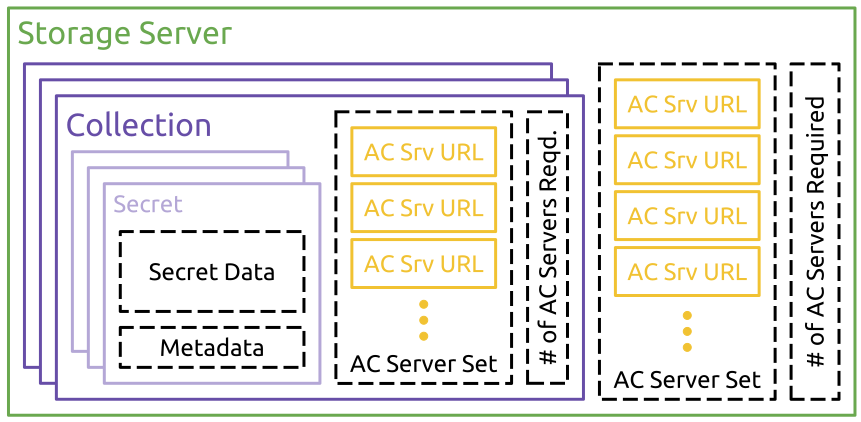
\includegraphics[width=\columnwidth]{./figs/pdf/datastructures-storage.pdf}
  \caption{Storage Server Data Structures}
  \label{fig:tutamen:storagestructs}
\end{figure}

The top-level data structure employed by storage servers is the
\textit{collection}. A collection represents a logical grouping of one
or more secrets (or parts of secrets). Associated with each collection
is a list of one or more access control servers delegated with
enforcing the access control requirements for the collection. Access
control granularity is thus set at the per-collection, not per-secret
level. A collection is also capable of storing user-provided metadata
to aid in the mapping of collections to the objects for which they
store secrets. Each collection stores one or more secrets or secret
shards. These secrets consist of the secret data an application wishes
to store and any associated user-provided metadata.\footnote{How best
  to map secret data to collections is left up to each
  application. This decision is primarily driven by the fact that
  access control is performed on the per-collection level. Thus, if an
  application requires that a set of secrets always have a common set
  of access control requirements, it is efficient to group these
  secrets into a single collection. In cases where each secret
  requires its own access control requirements (e.g., per-file
  encryption keys), it is appropriate for the corresponding
  application to store only a single secret per collection.}

\subsubsection{Access Control Protocol}
\label{sec:tutamen:arch:acp}

Access control servers control access related to both internal (i.e.,
access control server) and external (i.e., storage server) objects by
providing signed authorization tokens in response to valid
requests. Similar to previously proposed distributed and federated
access control systems~\cite{calero2010, leandro2012, neuman1994},
each authorization token grants the bearer a specific permission
related to a specific object. Unlike previous systems, however,
Tutamen is designed to avoid needing to trust any single access
control provider (see \S~\ref{sec:tutamen:arch:distributed}).
Figure~\ref{fig:tutamen:systembase} shows the basic communication
involved in the Tutamen access control process.

\begin{figure}[th]
  \centering
  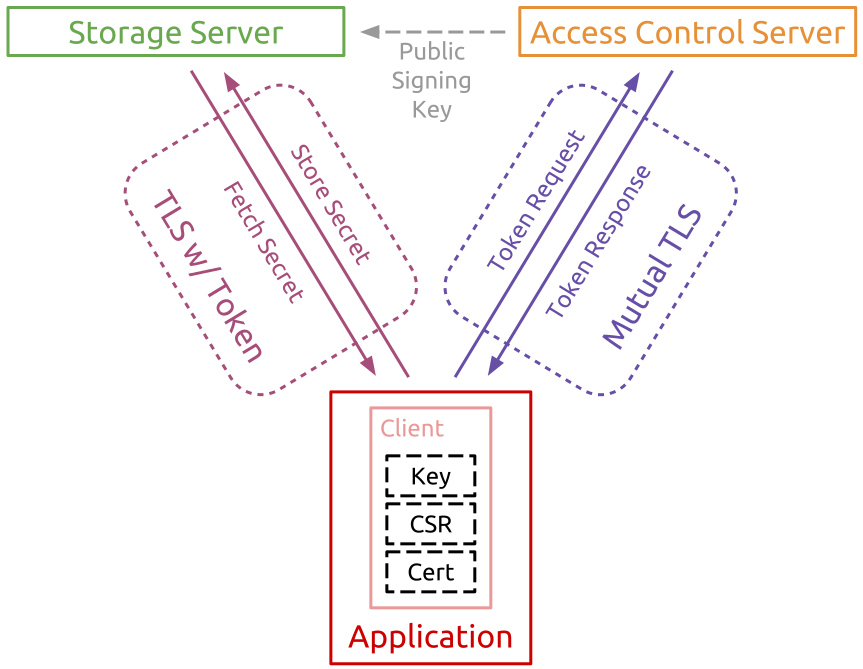
\includegraphics[width=\columnwidth]{./figs/pdf/system-base.pdf}
  \caption{Access Control Communication}
  \label{fig:tutamen:systembase}
\end{figure}

Each access control server generates authorization tokens in response
to a client sending an authorization request. Each authorization
request (and each corresponding token) includes two claims binding it
to a specific object: the object type and the object ID. Each token
request also contains a claim that binds it to a specific permission
for the corresponding object. Authorization requests are further bound
to the specific client making the request (authenticated via
mutual-TLS), and to an expiration time after which the token is no
longer valid. Tutamen allows the client to request a specific
expiration time for each token, facilitating the reuse of a single
token to repeat a specific action on a given object without needing to
re-authenticate each time. The access control server considers the
requested expiration time when deciding whether or not to approve an
authentication request, and may return an authorization valid for less
time than originally requested or deny a request for an overly long
duration altogether.

Upon receiving an authorization request from a client, the access
control server looks up the permission group for the corresponding
object (identified via the combination of object type and object ID)
and then loads the set of verifiers corresponding to the requested
permission. The server then traverses each verifier in this set,
checking for client membership in one of the accounts listed in the
verifier and executing any authenticator modules required by the
verifier until it finds (or fails to find) a verifier that is
satisfied by the request. If the server is able to verify compliance
with at least one verifier, it grants the authorization request and
returns a signed authorization token that includes the object type,
object ID, granted permission, and expiration time. The bearer of this
token presents it to either the access control server or a storage
server in conjunction with it's request to act on the corresponding
object.

Other than the bootstrapping operations and the token request
operations themselves, all requests to either storage or access
control servers must be accompanied by a valid token. The receiving
server validates this token using the public signing key of the
associated access control server. For requests to the access control
server itself, this key is available internally. For requests to
storage servers, the storage server downloads the signing key from
each delegated access control server. In this manner, access control
servers are responsible for granting and verifying authorization
requests, signing the corresponding tokens, and verifying tokens
accompanying requests to perform actions on ACS objects (e.g., to
create or modify verifiers or accounts). Storage servers are
responsible only for verifying tokens accompanying requests to perform
actions on storage objects (e.g., to create a collection or read a
secret).

\subsubsection{Distributed Usage}
\label{sec:tutamen:arch:distributed}

Tutamen is designed to be used in both centralized and distributed use
cases. The simplest Tutamen arrangement (e.g., as shown in
Figure~\ref{fig:tutamen:systembase}) involves leveraging a single
Tutamen access control server and a single storage server. In this
arrangement, a single storage server stores a complete copy of each
secret while a single access control server is charged with enforcing
access to these secrets. While this use case is easy to deploy, it has
two notable downsides. First, it forces the user to place a high
degree of trust in both the operator of the access control server and
the operator of the storage server. Second, it lacks any form of
redundancy. If either the access control server or the storage server
is unavailable, applications will be unable to retrieve any secrets.

A variety of systems have been proposed with the goal of minimizing
trust requirements for cloud infrastructure~\cite{bessani2011,
  kallahalla2003, kubiatowicz2000, mahajan2011,
  wilcox-o'hearn2008}. Tutamen applies similar ``minimal-trust'' goals
to the secret-storage problem by offering support for sharding secret
storage and access control duties across multiple servers. Operating
Tutamen in a distributed manner is largely a task that is pushed down
to the application (or client library). With the exception of offering
the necessary primitives to support such operation, both Tutamen
storage and access control servers are designed to be largely agnostic
as to whether they are being used in a centralized or a sharded
manner. This design has the benefit of avoiding server-side scaling
challenges, allowing the extra overhead required for distributed
operation to be supported by each application that requires it. This
design also helps avoid leaking unnecessary metadata to each Tutamen
server, making it harder for one server to identify (and thus attempt
to attack) the other servers involved in storing a single secret.

\begin{figure}[th]
  \centering
  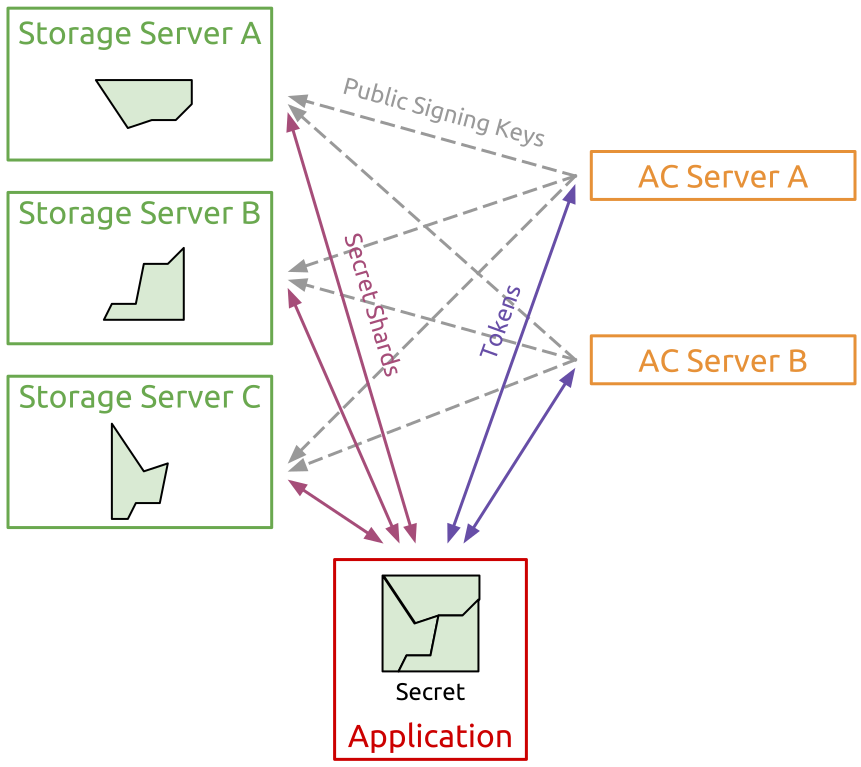
\includegraphics[width=\columnwidth]{./figs/pdf/system-distributed.pdf}
  \caption{Distributed Operation}
  \label{fig:tutamen:systemdistributed}
\end{figure}

Figure~\ref{fig:tutamen:systemdistributed} shows the basic layout of a
distributed Tutamen setup. In such a setup, the Tutamen application
first shards its secret using a $(k, n)$ threshold
scheme~\cite{krawczyk1993, shamir1979}, similar to previously proposed
systems~\cite{bessani2011, blaze1996, denning1996}. The application
chooses the value of $n$ based on the number of storage servers it
wishes to use. The value of $k$ is then chosen to control how many of
the servers must be available to retrieve the secret, or inversely,
how many server operators must collude to access a user's secret. The
application then pushes each shard to the $n$ storage servers. If the
application is merely concerned about storage redundancy, or about its
ability to trust a storage server operator, it can delegate the access
control for each secret shard to a single access control server. To
retrieve such a secret the application would request the necessary
token from the access control server and include it in its request to
each storage server for their respective shard of the secret. When the
application receives a response from $k$ of the storage servers, it is
able to reconstruct the original secret.

In most cases, however, the application will also wish to protect
itself against access control server trust and reliability
failures. This is accomplished via storage server support for the
specification of two pieces of metadata corresponding to each stored
collection: a set of AC servers approved to provide access control
tokens for the collection and a minimum number of servers from which
valid tokens must be received. These parameters form the basis of a
novel, yet simple, $(k, n)$ threshold scheme for access control
servers -- e.g., a collection may delegate a list of $n$ access
control servers from which an application must acquire at least $k$
valid tokens to gain access. Thus, if the user does not wish to trust
a single access control server, they may require tokens from at least
$k$ different AC servers to access the data stored in a given
collection. Likewise, if the application wishes to withstand the
failure of one or more AC servers, it can specify $n$ possible AC
servers where $n > k$.

To facilitate ease of management when operating in a distributed
fashion, Tutamen supports allowing applications to request use of
specific, randomly-generated UUIDs~\cite{leach2005} for each object at
creation time. This allows clients to use the same object ID across
multiple servers, alleviating the burden of maintaining a mapping
between object IDs and the servers to which they correspond. Using the
same object IDs across multiple servers also allows for more efficient
token management -- e.g., if an application uses the same collection
ID on three separate storage servers, all of which delegate a common
set of access control servers, it is possible (and desirable) for the
application to use a single token on all three servers.\footnote{The
  ability to request specific object IDs does have a downside: it
  opens Tutamen up to a possible denial-of-service (DoS) attack where
  an attacker attempts to request the object IDs they know another
  application wishes to use for themselves. Since each server may only
  use each object ID once, the first application to request a given
  UUID gets it. Thus, if an adversary knew which object IDs a given
  application planned to use, they could request these object IDs on a
  given access control server for themselves, depriving the original
  application of the ability to use those servers with that ID. At
  worst, however, this attack posses an inconvenience to applications,
  since an application is welcome to simply generate a new UUID for
  use with each object it stores instead.}

\subsection{Usage Example}

To illustrate the interaction of the various components of the Tutamen
platform, we present an example of the steps taken by an application
to store and then retrieve a secret via Tutamen. In this example, we
assume the application is using three storage servers and two access
control servers as shown in
Figure~\ref{fig:tutamen:systemdistributed}. We also assume the
application has already bootstrapped an account and an associated
client.

\begin{figure}[th]
  \centering
  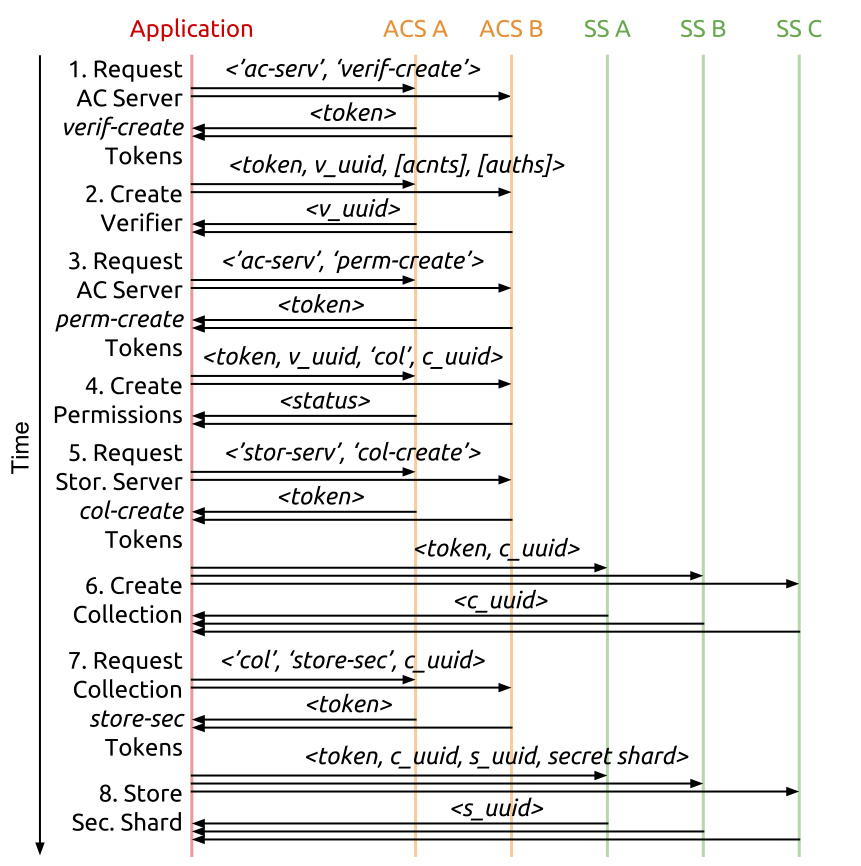
\includegraphics[width=\columnwidth]{./figs/pdf/store-secret.pdf}
  \caption{Storing a New Secret}
  \label{fig:tutamen:storesecret}
\end{figure}

Figure~\ref{fig:tutamen:storesecret} shows the steps required to
create a new collection and store a secret within it. We assume the
application has already sharded the secret into three parts -- one per
server.\footnote{Omitted from this diagram is the process of creating
  verifiers and permissions groups for the collection verifier
  itself. These objects are necessary to control who can read, modify,
  or delete the corresponding verifier after creation. The process for
  creating such objects is similar to the process of creating the
  collection-related verifier and permissions. To avoid the infinite
  recursion of needing verifiers for each verifier, it is possible for
  a verifier to be associated with a permissions group in which it is
  itself a member (i.e., a verifier can enforce its own access control
  specification).} As shown, the client starts by setting up the
necessary access control structures (i.e., a new verifier and a
corresponding set of collection permissions).\footnote{Note that it is
  critical that the client creates the permission set corresponding to
  the planned collection UUID prior to creating the collection
  itself. Failure to do so risks allowing another actor to ``hijack''
  the collection by requesting the permission set corresponding to the
  new collection's UUID before the original requester. As with other
  Tutamen operations, the first person to request an object
  corresponding to a given UUID gets it. Thus, a client should only
  create a collection using a given UUID after they have properly
  secured the corresponding permissions for the UUID in question on
  each AC server they wish to utilize.} Once the AC structures have
been created, the client creates the storage data structures: first a
new collection, than a secret within the collection. Prior to each
operation, the client must also request a token granting the necessary
permission from the AC server, meaning that about half the
interactions in the secret creation process are token requests.

\begin{figure}[th]
  \centering
  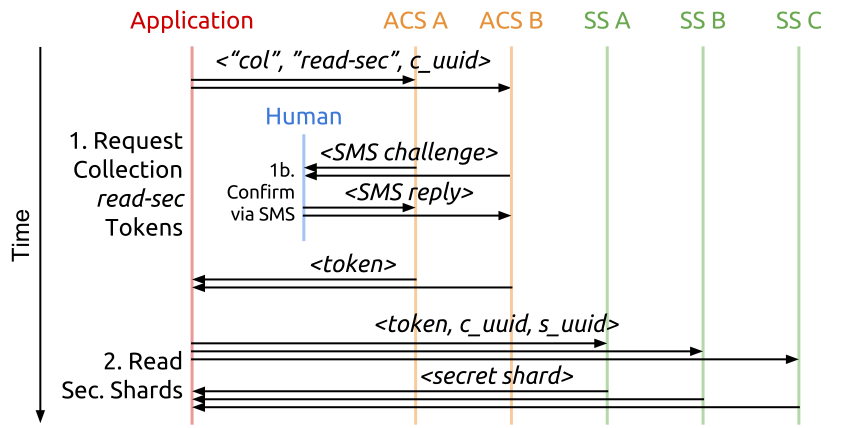
\includegraphics[width=\columnwidth]{./figs/pdf/fetch-secret.pdf}
  \caption{Retrieving an Existing Secret (w/ SMS Auth)}
  \label{fig:tutamen:fetchsecret}
\end{figure}

Figure~\ref{fig:tutamen:fetchsecret} shows the steps required to
retrieve an existing secret. This diagram also assumes that the secret
in question has an SMS (i.e. text message) authenticator associated
with it, requiring a user to provide a response to an SMS challenge in
order to approve access to the secret. Compared to the process of
storing a new secret, retrieving a secret is much simpler since it is
not necessary to create the slew of new access control objects
required when creating a new collection. Ignoring any round trips
required by individual authenticator modules (e.g., the SMS
verification), secret retrieval required only a single round trip to
each server: one to each AC server to retrieve a token and one to each
storage server to retrieve each shard of the secret. In Tutamen,
secret retrieval is thus less expensive than secret storage. We
foresee most secret-related workloads requiring many reads of a single
stored secret, so optimizing the system for reads over writes seems
appropriate.

\subsection{Implementation}

In order to demonstrate and test the Tutamen platform, we have created
reference implementations for the storage server, access control
server, and several client libraries. Our Tutamen server
implementation exposes a RESTful interface~\cite{fielding2000} for
both the access control and storage server APIs. This interface
accepts and responds using JSON~\cite{json} messages over the HTTPS
protocol. The full access control server API specification and
reference implementation are available
at~\cite{src-tutamen-apiaccesscontrol}. Likewise, the storage server
API specification and implementation can be found
at~\cite{src-tutamen-apistorage}. The prototype servers are written in
Python3 using the Flask web framework~\cite{python-flask}. Both
servers are served via WSGI~\cite{pep3333} using the Apache HTTP
Server~\cite{apache} for TLS termination and client-certificate
verification. Both Tutamen servers rely on a shared
\texttt{pytutamen-server}~\cite{src-tutamen-pytutamenserver} Python
library for the implementation of their core logic. This library
leverages the Redis~\cite{redis} key-value store for persistent
storage. Our Tutamen implementation adopts the JSON Web Signature
(JWS)~\cite{rfc7515} and JSON Web Token (JWT)~\cite{rfc7519}
specifications for exchanging cryptographically authenticated tokens
between Tutamen applications, access control servers, and storage
servers. We leverage the pyjwt~\cite{pyjwt} library for JWS and JWT
support. These tokens are then attached to subsequent requests using a
custom HTTP header field.

The access control servers expose a pluggable authenticator interface
through which end users and other developers may add custom
authentication functionality. This interface is primarily designed to
allow users to specify authentication checks beyond the client
certificate authentication automatically performed on every
request. As an example, we have implemented an authenticator module
that allows users to approve Tutamen token requests via SMS text
message using the Twilio~\cite{twilio} messaging platform. We also
envision authenticator modules for enforcing access control rules such
as only allowing requests during certain times of day or from specific
network addresses. Each authenticator plugin is provided with both a
set of per-instance configuration data (e.g., to whom an SMS message
gets sent for approval) and all of the details of a specific token
request (e.g., IDs and metadata associated with the requesting account
and client, from which information such as originating IP address or
time of day can be extracted).

In addition to the server and authenticator implementations, we have
also created reference Tutamen client libraries for both
Python~\cite{src-tutamen-pytutamen} and
Go~\cite{src-tutamen-go}. Using the Python client library, we have
created a Tutamen CLI application through which users may directly
store and retrieve secrets and control secret sharing and access
control rules~\cite{src-tutamen-cli}. The CLI is useful for managing
Tutamen objects even in cases where other applications (see
Section~\ref{sec:apps}) are set up to interface directly with the
Tutamen platform. In this manner, it is not necessary for every
Tutamen application to implement all Tutamen management
functionality. Instead, an application might leverage only the
necessary Tutamen commands to perform secret-storage and retrieval,
leaving the task of managing the access control of Tutamen-stored
secrets to the CLI or to another dedicated management application.

%%  Localwords:  Tutamen ACS HTTPS CSR CSRs Authenticators verifiers
%%  LocalWords:  authenticators authenticator Custos
%%  LocalWords:  DoS SMS Redis AGPLv JWS JWT pyjwt pytutamen LGPLv
%%  LocalWords:  Twilio tutamen Auth

\section{Security and Trust}
\label{sec:trust}

One of Tutamen's primary design goals is its ability to support a wide
range of security and trust requirements. It achieves this goal
through its support for both centralized and distributed operation as
well as though its support for a range of authentication mechanisms.

\subsection{Security of Individual Servers}

The Tutamen security model is rooted in the security of the access
control servers. If the operation of these servers is secure, the
operation of the rest of the system may also be secure. Any security
guarantees provided via the access control server are extended to the
storage servers via the signed tokens the AC servers provide.

The security of each individual access control server rests on several
requirements. Failure to uphold these requirements will result in the
failure of an security guarantees provided by the AC server.

\begin{packed_desc}
\item[Certificate Authority Role:] Each access control server acts as
  a CA delegating with issuing and verify client certificates for each
  of its registered clients. Thus, its important that the CA keys
  stored by each AC server remain secure and that each CA server
  faithfully verifies the certificate presented by each client
  connection. Failure in either of these roles will result in a
  failure of any security guarantees provided by the AC server.
\item[Token Issuance and Verification:] Each access control server is
  responsible for verifying the access control requirements bound to
  specific object/permission combinations, issuing signed tokens
  attesting to such verification, and verify the signatures of tokens
  the tokens it receives from clients wishes to operate on access
  control objects. As such, it's important that each AC server keep
  its private token signing key secure and that if faithfully verifies
  both the access control requirements governing specific token
  requests as well as the signatures on all incoming tokens.
%\item[Collision Security:]
\end{packed_desc}

The storage servers must uphold the following security
requirements. Failure to do so results in a failure of the security of
the storage server.

\begin{packed_desc}
\item[Token Verification:] Each storage server must faithfully obtain
  the public token signing key from each AC server delegate to provide
  access control for a given storage object. The storage server must
  then use these keys to verify the signatures on all tokens it
  receives. Assume the token signatures is valid, the storage server
  must faithfully enforce the claims asserted in a given token:
  e.g. by only allowing actions granted by the permission contained in
  the token on the object the token identifies prior to the expiration
  time specified by the token.
\item[Secure Storage:] Each storage server must take steps to store
  user-provided secrets in a secure manner, releasing them only to
  requests accompanied by a valid token granting such release.
\end{packed_desc}

Since the tokens the storage server must verify are provided by the AC
servers, the security of the storage server with respect to a given
collection is dependent on the security of any designated AC servers
associated with said collection. If these AC servers are insecure, the
storage server will not be secure.

The security of Tutamen also, in most cases, depends on the security
of the public CA/PKI system. While AC servers act as local CAs for the
purpose of issuing and verify client certificates, we believe that in
most cases both Tutamen AC and storage servers will rely on public CA
system for obtain server certificates verifying the mapping between
DNS names and the server itself -- as do most public websites. Since
Tutamen storage servers retrieve the correct signing keys form each AC
server on the basis of the AC servers domain name, properly verifying
this name is critical. Similarly, its important for clients to verify
they are talking to the storage and AC servers they intend to, and
verifying the server certificates of each of these servers via the
standard TLS handshake process if thus also critical.

%Todo: cite other TLS security efforts such as CT, etc?

\subsection{Security of Multiple Servers}

Unlike existing secret management systems~\cite{vault, confidant,
  keywhiz}, the Tutamen architecture is capable of remaining secure
even when individual storage or access control servers fail to meet
their security requirements. Such failures may result from physical
server compromise, software bugs, malicious intent or incompetence on
the part of the server operator, or compelled failures.\footnote{For
  example, being forced to turn over stored secrets in response to
  legal or governmental pressure.}

To work around security failure of individual server, Tutamen
applications can leverage Tutamen distributed operation modes. In
these modes, the security of the system as a whole is diffused -- no
longer relying on the security of any specific access control or
storage server in order to keep an applications' secrets secure. As
described in Section~\ref{sec:tutamen:arch:distributed} each
applications can distribute both secrets storage and access control
delegations using $n$ choose $k$ schemes. In such setups, the
difference between n and k represents the degree to which a Tutamen
applications can withstand security failures of the deploys AC and
storage servers. For example, an applications which chooses to shard
its secrets across five storage servers where any three shards are
sufficient to recreate the secret ($n=5$, $k=3$) will continue to
remain secure even if two of the storage servers fail to meet their
security obligations. Similarly, if each secret shard delegates five
possible AC servers, tokens from three of which are required to grant
secrets access, the applications can withstand the failure of two AC
server to uphold their security guarantees. Since the security of each
storage server is dependent on the security of the associated AC
servers, in most cases\footnote{There may be cases where a user
  happens to trust the AC servers more than the storage servers that
  would justify having a larger $k-n$ storage delta than the $k-n$
  access control delta.} there is no security benefit from having a
greater $n-k$ delta for storage servers than for AC servers (although
such a delta may still yield reliability benefits).

\subsection{Trust Model}

Trust in Tutamen follows from the security models of both individual
Tutamen servers and of the distributed Tutamen deployment
architectures. If a Tutamen applications is leveraging only a single
storage and AC server, the applications is placing a high degree of
trust in both servers (and by proxy, the operators of both
servers). This level of trust may be appropriate for some use cases --
e.g. when a user is operating their own Tutamen's servers, but is
often inappropriate in many other cases (e.g. when using third party
hosted Tutamen servers). Fortunately, Tutamen also allows applications
to avoid placing a high degree of trust in any single server by
leveraging multiple servers and picking $k$ and $n$ in a manner that
corresponding to the degree by which server is trusted.

Beyond minimizing the amount of trust placed in each Tutamen's server
by leveraging multiple servers, we also envision economic incentives
helping to ensure Tutamen server trustworthiness. The Tutamen protocol
is standardized and designed to support a range of interchangeable AC
and storage server providers. Such a design allows for the development
of a Tutamen server marketplace where both AC and storage server
providers can compete against each other on the basis of
trustworthiness, features (e.g. what types of authenticates they
support), and cost. In such an ecosystem, Tutamen service providers
who fail to uphold the Tutamen security requirements on their servers
will suffer a negative economic effect, incentivizing such
behavior. Its also likely the storage providers who take additional
steps to protect the secrets they store (e.g. by using system such as
Trusted Platform Modules (TPM) to encrypt the secrets they hold and
harden server security) would be able to command a higher price in the
marketplace,incentivizing such best practices.

Thus, unlike other third-party cloud services where faithfulness to
customer desires and economic incentives are in direct competition
(e.g. as is the case on many ``free'' third part services that depend
on selling user data to advertisers in order to generate revenue),
Tutamen encourages a system where economic incentives are well aligned
with applications security. That fact, coupled with the high degree of
control over third-party trust Tutamen grants to each application by
allowing each application to select both the number of and which
servers the application wishes to use, make Tutamen a failure robust
system in the face to both security and trustworthiness failures. Such
robustness is a critical component if any successful security storage
system.

%\subsection{Discussion}


%%  LocalWords:  Tutamen's Tutamen CAs DNS

\section{Applications}
\label{sec:apps}

Tutamen is designed to support a wide range of applications. We have
integrated our reference Tutamen design with a set of common
applications for the purpose of demonstrating the value derived from
using a secure storage system such as Tutamen. These applications all
leverage Tutamen's flexibility to achieve functionality that would
have been difficult or impossible to achieve without using a system
like Tutamen.

\subsection{Block Device Encryption}

Block device encryption systems are a popular means of protecting the
data stored on computing systems in the event that the system is lost,
stolen, or otherwise physically compromised.  Block-level encryption
systems such as dm-crypt~\cite{dm-crypt} (generally coupled with the
Linux Unified Key Setup (LUKS)~\cite{luks} container) or the
QEMU~\cite{qemu} qcow2 encryption system provide methods for securing
the data stored on laptops, desktops, and VMs. Such systems
traditionally bootstrap security by requiring the user to enter a
password at boot-time to unlock a locally stored encryption key which
is then used to decrypt the block device in question. Unfortunately,
the ``human-at-keyboard'' security root make such systems difficult or
impossible to use atop headless servers or in related situations where
no human can be expected to be present at boot-time. We've leveraged
Tutamen to overcome this barrier.

To add Tutamen-support to LUKS/dm-crypt we've created a Tutamen-aware
implementation~\cite{src-tutamen-askpassword} of the \texttt{systemd}
Password Agent Specification~\cite{systemd-passwordagents}. This
specification is used by LUKS/dm-crypt \texttt{cryptsetup} utility to
request the necessary decryption secret. At boot time,
\texttt{cryptsetup} will send out a request for this secret. Normally
this triggers a ``human-at-keyboard'' prompt for a boot
pass-phrase. Our Tutamen-aware password agent can instead respond to
such requests by retrieving the necessary decryption secret from a
Tutamen storage server (after first retrieving the necessary tokens
from the corresponding Tutamen AC server). In addition to modifying
the ask-password utility, we made several modifications to the
\texttt{initrd} creation process to add Tutamen networking support,
the necessary Tutamen client TLS key pair, and a config file
specifying which Tutamen servers to use and the UUIDs of the relevant
Tutamen collection and secrets.

We've also integrated Tutamen support with QEMU to provide qcow2
encryption keys when a VM boots~\cite{src-qemu-tutamen}. Similar to
the dm-crypt setup, QEMU normally requires the user to provide the
encryption key via the QEMU console when a VM launches. Our system
replaces this ``human-at-keyboard'' process with Tutamen-based secret
retrieval. In addition, QEMU currently requires the user to provide
the full encryption key, not just a pass-phrase to unlock a pre-stored
key~\cite{berrange-qemucrypto}. This has negative security
repercussions in the common case where users pick short password-like
keys. Using Tutamen, we can overcome this barrier since Tutamen
servers have no qualms about needing to store or remember sufficiently
long encryption keys. Our system thus increases both QEMU's security
and its ease of use.

Using these setups, we're able to boot servers and VM images with
encrypted disks without requiring a human to be physically present at
the machine. In cases where we still desire human approval of the boot
process, we can leverage our SMS authenticator module to get an
on-demand confirmation from a designated human as a prerequisite to
Tutamen releasing the correct key. This allows us to gain the same
level of human-in-the-loop security provided by a typed pass-phrase,
but without actually requiring a human to go to the datacenter to type
one in. In situations where we don't desire a human-in-the-loop at
all, we envision automating the approval process via the use of
time-of-day and IP-source authenticators.

\subsection{Encrypted Cloud File Locker}

Cloud-based file lockers such as Dropbox~\cite{dropbox} are extremely
popular today. Unfortunately, these systems require users to trust the
cloud provider with full access to their (generally unencrypted)
data. Users wishing to overcome this deficiency can optionally encrypt
all of their data on the client before syncing it to the file locker
provider, but doing so does not generally interact well with such
services' sharing and multi-device use cases, requiring users to
employ manual, out-of-band key exchange mechanisms to share or sync
their encrypted files. We don't believe file locker users should have
to choose between easily syncing or sharing their files and using
encryption to protect their data.

Tutamen provides a solution to this problem by offering a secure
key-sharing mechanism. Instead of manually distributing or sharing
encryption keys, the user can store their key as a Tutamen secret and
leverage Tutamen's access control features to share the secret with
the accounts of their friends. This entire process could even be
automated such that when a user shares a file via Dropbox, the
corresponding encryption key is automatically shared via Tutamen.

Toward this end, we have created FuseBox: an alternate Dropbox client
that performs client-side encryption of all Dropbox files, storing the
corresponding encryption keys on our reference Tutamen server. FuseBox
achieves goals similar to those achieved by~\cite{goh2003}, but
without requiring out-of-band key management. Similar to other
file-system-level encryption systems~\cite{blaze1993, Cattaneo2001,
  halcrow}, FuseBox provides transparent file encryption to end
users. In order to avoid the storage space and security challenges
presented by locally caching all Dropbox data (i.e., the operation mode
for the official Dropbox client), FuseBox uses AES~\cite{daemen1999,
  nist2001} as a stream cipher to transparently stream and encrypted
data to/from Dropbox's servers on demand.  The source code for our
FuseBox implementation is available at~\cite{fusebox}.

Since FuseBox leverages Tutamen to store each per-file encryption key,
it becomes possible to share an encrypted file via Dropbox, share its
encryption key via Tutamen, and achieve the same level of
functionality traditional Dropbox users have without having to expose
one's data to Dropbox. While the key sharing process in FuseBox is not
yet directly synced with Dropbox's file sharing system, the Tutamen
CLI can be used to quickly share the encryption keys between users. In
this manner, we've used FuseBox to store and share encrypted files
with nearly the same ease with which one might use the traditional
unencrypted Dropbox client. By leveraging Tutamen, FuseBox also gains
the ability to remotely revoke file access, e.g., in the case a device
is lost or stolen, similar to systems such as~\cite{geambasu2011}. We
also have plans to add cryptographic file authentication to FuseBox's
streaming architecture using techniques such as those described
at~\cite{McGrew2005}. FuseBox, via Tutamen's distributed operation
mode, also avoids the sharing pitfalls associated many existing
``secure cloud storage'' providers~\cite{wilson2014} by avoiding
reliance on a single trusted party to facilitate sharing operations.

\subsection{Other}

Since our Tutamen-capable ask-password port speaks the standard
systemd Password Agent protocol, it can also be used to provide
Tutamen-backed pass-phrase storage to any applications leveraging this
protocol, including OpenVPN and various password storage utilities. We
have not yet thoroughly explored these use cases, but we envision a
Tutamen-passed systemd password agent being useful in a wide range of
situations beyond just full disk encryption. Our experience
integrating the systemd password agent with Tutamen also suggests that
Tutamen would provide a useful backend for a variety of other
``agent'' protocols (e.g.,~\cite{cox2002, ylonen1996}).

%%  LocalWords:  Tutamen keyslots keyslot systemd cryptsetup initrd
%%  LocalWords:  libcryptsetup initramfs Archlinux RedHat ini pid FDE
%%  LocalWords:  dgram tutamen OpenVPN TUTATEM luks authenticators dm
%%  LocalWords:  SMS authenticator golang Tutamen's FuseBox FuseBox's
%%  LocalWords:  QEMU qcow

\section{Evaluation}
\label{sec:eval}

\begin{figure}[th]
  \centering
  \includegraphics[width=\columnwidth]{./figs/png/chart-combined-timings.png}
  \caption{Timings for Tutamen Operations}
  \label{fig:eval:timings}
\end{figure}

\begin{figure}[th]
  \centering
  \includegraphics[width=\columnwidth]{./figs/png/chart-iops.png}
  \caption{Throughput vs Latency}
  \label{fig:eval:iops}
\end{figure}

\subsection{Usage}

\subsection{Discussion}

\section{Conclusion}
\label{sec:conclusion}

How best to securely store secrets is a pressing issue in today's
cloud-oriented, third-party-hosted, ephemeral-infrastructure-based
environment. This need has triggered the creation of several
secret-storage frameworks and systems. Unfortunately, these existing
systems prove deficient in at least three key secret-storage
capabilities: the ability to support operation outside of a single
administrative domain, the ability to operate atop untrusted
infrastructure, and the ability to support a wide range of access
control use cases.

We created Tutamen to demonstrate our concept for a next-generation
secret-storage system. Tutamen supports client-controlled secret
sharding to allow applications to leverage minimally-trusted server
infrastructure. Tutamen also supports a flexible and modular
authentication mechanism that allows end users to specify complex
access control requirements. We've successfully coupled Tutamen with a
number of applications, including full disk encryption on headless
servers and client-side encrypted file sharing between multiple
parties. These use cases would be difficult (or at least burdensome)
to realize without a system such as Tutamen.

We plan to continue developing the Tutamen ecosystem. On the
server-side, we have plans to work toward increased performance and to
add support for additional authenticator modules. While the Tutamen
servers currently have basic logging support, we also plan to expand
this support, and to explore interfacing Tutamen audit logs with
intrusion detection systems in order to expose more actionable
intelligence to Tutamen authenticator modules. We are also considering
tying Tutamen's logging infrastructure to a public audit system
similar to~\cite{laurie2013}. Such a system would help to further
reduce the trust Tutamen users must place in individual Tutamen
servers by exposing mechanisms by which a user could reliably audit
the behavior of such providers.

We have made all of the Tutamen source code available via the
previously referenced repositories. We encourage others to experiment
with our Tutamen prototype and reference implementation, or to
integrate Tutamen with their projects or applications. We hope that
Tutamen (or similar distributed secret-storage systems) can help to
ease the secret-storage burden currently imposed on administrators,
developers, and end users by providing an alternative to manually
managing sensitive secrets in a manner that also minimizes third party
trust.

%%  LocalWords:  Tutamen authenticator Tutamen's


{
%  \clearpage
%  \footnotesize
  \bibliographystyle{abbrv}
  \bibliography{refs}
}

\end{document}

%%  LocalWords:  Tutamen Tutamen's
